%!TEX root = pfe-book4.tex
%!TEX TS-program = pdflatex
%!TEX encoding = UTF-8 Unicode


\cleardoublepage
%\mainmatter
\chapter[Generalizations of Mechanics]{Generalizations of \\Mechanics}
\label{ch-04}

\section{Relativistic Mechanics}

Newtonian mechanics that we discussed in the first book of this series is one of the greatest achievements of the human genius. It made it possible to compute the paths of planets, the trajectories of rockets and spacecraft, the behaviour of mechanisms. The development of phys­ics in the twentieth century demonstrated that the laws of Newtonian mechanics have two limitations: they be­come unsatisfactory when dealing with the motion of particles of small mass and they fail us when we have to do with the motion of bodies with velocities close to the velocity of light. For small particles, Newtonian mechanics is replaced by the so-called \emph{wave mechanics}; for fast bodies, it gives way to \emph{relativistic mechanics}.

Classical mechanics is also made more complicated when we encounter very great forces of gravitation. The unimaginably strong fields of gravitation that govern the behaviour of superdense stars force us beyond the limita­tions of such simple formulas of mechanics as were ex­plained in the first book. We will not dwell on such changes here but will take up the two highly important generalizations just mentioned when dealing with the motions of microparticles and when studying velocities comparable to the velocity of light.

Let us begin with relativistic mechanics. The path leading to this important division of physics least of all resembles a straight road. Not only is it tortuous but it even passes through quite different countries. The starting point here is the ether. Generally speaking, physicists were having it easy at the end of the 19th century. Max Planck's teacher did not advise him to take up physics because that science, he said, is practically completed. There were only two slight blemishes on the otherwise perfect edifice of physics: drawbacks in accounting for the radiation of a black body (when that was cleared up, physicists discovered the quantum) and the distressing experiment of Michelson. This experiment, which proved that the velocity of light does not combine with the velocity of the earth in its orbital motion and is the same in all directions, caused some anxiety about the properties of the ether.

Hardly anyone doubted the existence of some kind of delicate matter whose oscillations constituted the electromagnetic waves. After over a hundred years have passed it seems even surprising that despite the great number of inconsistencies that the ``ether'' hypothesis led to, the vast majority of scientists -- some extremely talented -- went to great lengths to introduce no end of supple­mentary assumptions with the sole purpose of salvaging the concept of light as the motion of an invisible ultimate material substance.

\newpage
\begin{center}
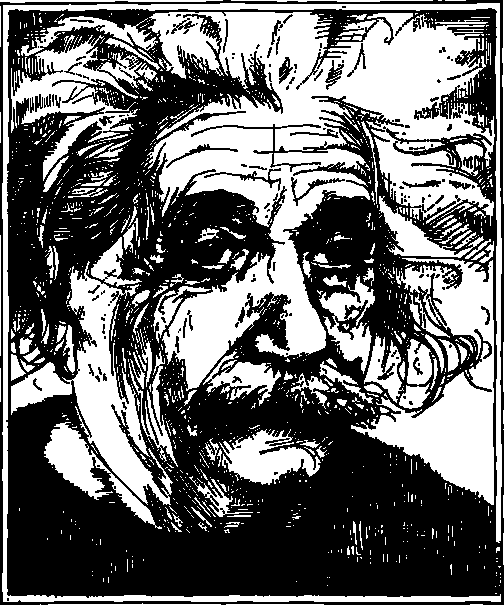
\includegraphics[width=0.8\textwidth]{figures/einstein.pdf}
\end{center}
{\small \textsf{{Albert Einstein [1879-1955]}} -- \textsf{\footnotesize the genius who created the theory of relativity and revolutionized all physical thinking. In 1905, Einstein published a treatise devoted to the special theory of relativity. In 1907, he obtained a formula relating energy and the mass of a body. In 1915, Einstein published his general theory of relativity. From this theory there followed new laws of gravita­tion and conclusions concerning the curvature of space. The theory of relativity does not exhaust Einstein's contribution to physics. From the research of Max Planck he drew the conclu­sion that there exists a light particle (called a photon) and demon­strated that from this standpoint it is possible to account for a number of fundamental phenomena, including the photoeffect.}}

Some pictured the ether as a placid sea through which the planets moved; others thought that the ether could be entrained like air by moving bodies. As strange as it may now seem, nobody suggested the obvious idea that the oscillations of electric and magnetic vectors occur \emph{at a point}, and for that reason cannot be accounted for in terms of mechanical displacements. Every effort was made to hold onto the old concepts, theories were set forth in which formally proper mathematical expressions
were derived (the infamous square root $\sqrt{ 1- (v/c)^{2}}$ includ­ed as well; here $v$ was the velocity of a body and $c$ the velocity of light), but the equations were wrongly interpreted. Particularly upsetting was the Michelson experi­ment, first carried out in 1881. Using an interferometer (described in \hlgray{Chapter \ref{ch-02}}), Michelson demonstrated that the velocities of light along and across the orbital motion of the earth are practically the same.

Even this fact (completely upsetting the theory con­cerning the existence of an ether) did not compel leading physicists to give up faith in a tenuous matter permeating all bodies. Michelson's experiment forces us to give up any idea of an ethereal wind? Good and well, we will give up the wind and the universe will be still more beautiful with a motionless ether, and we will accept the Newtonian absolute space with respect to which all celestial bodies move.

To account for the Michelson experiment, such outstand­ing physicists as Sir Joseph Larmor (1857-1942) and Hendrik Antoon Lorentz (1853-1928) applied the hy­pothesis of the contraction of bodies in the direction of their motion. However, logical inconsistencies and the artificial nature of the explanations of many phenomena concerning electrodynamics continued to leave a sense of inadequacy.

The Gordian knot of contradictions was finally cut by the greatest physicist of our century, Albert Einstein (1879-1955).

The starting point in Einstein's reasoning was the principle of relativity. There was hardly any doubt in anyone's mind, after Galileo, that in regard to mechani­cal motions, all inertial systems are equivalent (please turn back to book one in this series and review the facts about inertial systems). What appeared to be rather strange and esthetically unpleasant was that we have equivalence for mechanical motion but not for electromag­netic phenomena. Now suppose we assume the principle of relativity to hold true for all phenomena. But doesn't that lead to a contradiction? Imagine a source emitting a light ray. The light wave sets out into space and, observing it, I permit myself to disregard the fact that the source may be in motion or at rest. But if that is so, then the velocity of electromagnetic waves (\SI{299 792}{\kilo\meter\per\second}) must be the same from the viewpoint of observers living in systems moving with respect to one another with an arbitrarily high velocity $v$.

Suppose we have a train on a straight section moving at a constant speed of $v$. Parallel to the track is a highway and on it and moving in the same direction is a speeding motorcyclist. A traffic officer sees the culprit and with his miniature radar quickly finds that the motorcycle is doing \SI{85}{\kilo\meter\per\hour}. The locomotive engineer glances at the motorcyclist and sees him catching up with the train and then overtaking it. This observer has no difficulty in measuring the speed of the motorcycle. It is $u' - \SI{35}{\kilo\meter\per\hour}$. It is obvious that the speed of the train is \SI{50}{\kilo\meter\per\hour}. The law of composition of velocities holds true:
\begin{equation*}%
u = v + u'
\end{equation*}
This most obvious of all rules does not fit the case of light rays. Photons move with the same velocity with respect to two observers located in different inertial sys­tems.

The genius of Einstein lay in the fact that he rejected this most obvious conclusion not only for light but, aiming to retain a unified approach to all physical phe­nomena (both electromagnetic and mechanical), was so bold as to give up the law of composition of velocities for all bodies.

From this standpoint, there is no need to explain anything in Michelson's experiment. Since the velocity of light does not depend on the velocity of motion of the source, it (the velocity) will be the same in all directions: both along the earth's orbit and across the orbital path of the earth around the sun.

It follows immediately from the principles just for­mulated that the velocity of light is the maximum veloc­ity.\footnote{Generally speaking, however, relativistic mechanics is not con­tradicted by the existence of particles moving with velocities arbitrarily greater than the velocity of light. Theoreticians have even given them a name: they are called \emph{tachyons}. However, if such particles existed, the velocity of light would still be a limiting velocity for them -- it would be the minimum veloc­ity not the maximum velocity. I personally think that the theory of tachyons is nothing more than an elegant mathematical toy. If the world of tachyons did indeed exist, then events taking place in the universe would, in principle, never be influenced by that world.} Indeed, if the velocity of light is never combined with the velocity of any source, that means it is impossi­ble to overtake light. In his reminiscences, Einstein recalls that as early as 1896 he was considering the following question: ``If it were possible to set out after a light wave with the velocity of light, then would we be dealing with a time-independent wave field? That does indeed seem to be impossible.''

To summarize, then: there is no particle that can move with a velocity greater than the velocity of light. Let us give some thought to this statement. It is so paradoxical that it needs repeating. If an electromagnetic wave takes off from the earth or another planet in some direction, then the rate of propagation of that wave, when mea­sured by a terrestrial observer and by an observer flying over the earth in a spacecraft moving with a fantastic velocity, is the same. This assertion holds true also for any particle moving with a velocity equal to the velocity of electromagnetic waves. Light is no exception in the Einstein theory.

Now what happens when the velocity of a moving body is less than the velocity of light? Obviously, in this case too the simple principle of the composition of velocities that is so usual does not hold true. However, the devia­tion from the ordinary rule for composition of velocities begins to be felt only when the velocity of the body is very great.

\emph{Relativistic mechanics} -- that is the name given to the mechanics of fast-moving bodies -- leads to the following rule for the composition of velocities:
\begin{equation*}%
V = \frac{v + v'}{1 + \dfrac{vv'}{c^{2}}}
\end{equation*}
Make a rough estimate of what the values of $v$ and $v'$ must be for corrections to the simple rule for composition of velocities to be needed.

How about spaceflight? Does the ordinary rule for the composition of velocities function when we deal with speeds of tens of kilometres per second?

We know that a good way to gain speed is to launch a second rocket system from a spaceship in flight. This could be one way of launching spacecraft to the outer reaches of the solar system. Denote by $v$ the velocity of the space­ ship relative to the earth, and by $v'$ the velocity of the craft launched from the spaceship relative to the space­ ship. Suppose both velocities, $v$ and $v'$, are equal to \SI{10}{\kilo\meter\per\second}. Now compute the exact velocity of the spacecraft relative to the earth, using the exact formula of the composition of velocities. To the 1 in the denominator we have to add the fraction $\num{d2}/(\num{9d10})=\num{d-9}$. The correction is practically negligible, which means the classical rule for the composition of velocities holds true. 

The question now is: When does relativistic mechanics come into its own? We will have the answer soon, but meanwhile let us continue the consequences that stem from the hypotheses just formulated. Since we are forced to give up the principle of composition of velocities, we must be ready to introduce essential corrections in
the other formulas of mechanics as well.

As we have already mentioned, it was Michelson's experiment that played a decisive role in the development of the theory of relativity. Michelson demonstrated conclusively that the velocity of light along the earth's orbit and across it is the same.

We will not consider the path of rays in the Michelson interferometer and will confine ourselves to simpler events. Somewhere on the earth, a very simple laser experiment is set up on a tower at an altitude $l$ above the earth's surface. The ultrafine laser beam goes in the direction of the earth's radius, is reflected from a mirror placed on the earth's surface, is returned to where it started from, and is received by a photocell that engineers place in such a position that we regard the light source and the receiver of light to be in a single point. In \figr{fig-4.1} it is labelled $S$. Using an ultrarefined stopwatch, we can fix two instants: the first when the light set out and the second when it reached the photocell.

%\clearpage

\begin{figure}[!h]
\centering
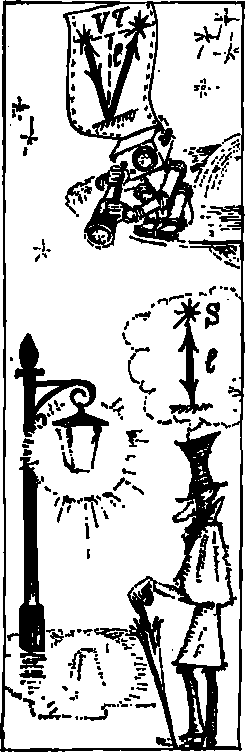
\includegraphics[width=0.4\textwidth]{figures/fig-04-01.pdf}
\caption{A simple experiment to prove constancy of velocity of light.}
\label{fig-4.1}
\end{figure}


Two observers follow this event. The first one stands next to the experimental setup, the other one is perched on a distant star. Both observers measure the time interval $\tau$ between the two events: the emission of light and its return to point $S$. The first draws the path of the ray and it turns out to be simplicity itself. He believes that the paths of the ray there and back coincide absolutely. His reasoning is corroborated by the equation $\tau =2l/c$.

The stellar observer follows the flash as the light starts out on its journey and records its arrival at the photocell.

The time interval that he measures is equal to $\tau$. To be sure everything is properly done, he too draws the path of the ray. For him, however, the positions of point $S$ at the time the stopwatch was switched on and the instant he recorded the reaction of the photocell do not coincide. The path of the light ray in his case is different. The stellar observer knows the velocity of the earth relative to himself and so what he gets is an equilateral triangle, the base of which is equal to $v \tau$ and the altitude to $l$. Using the Pythagorean theorem, the stellar observer finds that the path traversed by the light ray is equal to $2 \sqrt{ l^{2}+ (v\tau/2)^{2}}$. This path is equal to $c \tau$ , because the ve­locity of light is the same for all observers. If that is so, the time interval between the two instants is equal to
\begin{equation*}%
\tau = \frac{2l}{c \sqrt{1 - \dfrac{v^{2}}{c^{2}}}}
\end{equation*}
That is a surprising result! From the standpoint of the terrestrial observer, the same time interval between those very same events is equal to $2l/c$.

Appealing to logic, we can draw an unavoidable con­clusion: the time reckoned by an observer at rest differs from the time reckoned by an observer in motion.

The time of the stationary observer is called the \emph{prop­er time} and is denoted by $\tau_{0}$. We find that the time of an observer moving with velocity $v$ is connected with the proper time by the expression
\begin{equation*}%
\tau = \frac{\tau_{0}}{\sqrt{1 - \beta^{2}}}, \,\,\textrm{where}\,\,\beta = \frac{v}{c}
\end{equation*}
What this means is that a moving clock goes more slowly than a stationary clock. If we accept the basic postulates of the theory, we cannot escape such a conclusion. And this leads to the strange, at first glance, consequence that the idea of simultaneity has to be given up.

But won't it turn out, then, that from the viewpoint of one observer, Jim fired a gun and John was killed by the bullet while, from another point of view, John was killed first and Jim fired later? The reader can rest assured that relativistic mechanics does not allow for any such nonsense. The principle of causality will never be upset. And the proof can even be given popularly, but, unfortunately, that is beyond the scope of this book.

However, a few words are in order about the so-called twin paradox which even now is brought forth as proof of the inconsistency of the theory. John and Pete are twins. Pete takes leave of John and sets out on a space voyage with a velocity close to the velocity of light, and after a certain time returns to earth. Pete's clock has been going slower and so he returns to earth still fresh and young, whereas his brother John has grown old and feeble.

However -- fortunately or unfortunately, depending on who likes what -- no such meeting can be organized, that is, if we keep to the conditions under which the formulas under discussion hold true. The point is that Pete would have to reverse his velocity, and so the conclusions re­ferring to inertial systems have nothing to do with this case.

The relativity of time is not the only consequence of the new theory. Just as the proper clock of the observer goes faster than any other clock, so also the length of a rod, $l_{0}$, held in one's hand is the maximum length. From the point of view of any observer moving with velocity v along the rod, that same length is equal to
$l_{0}\sqrt{1 - \beta^{2}}$.

The same root also appears in the expression for the mass. The mass $m_{0}$ of the body that the observer holds in his hands is termed the \emph{rest mass}. It is minimum. For a moving observer,
\begin{equation*}%
m = \frac{m_{0}}{\sqrt{1 - \beta^{2}}}
\end{equation*}
It is quite natural that the mass increases with an increase in velocity. Indeed, if velocity has a limit, then as a particle approaches that limit, it becomes progressively more difficult to accelerate the moving particle. That is precisely what is meant when we say that the mass of the particle increases.

For a long time, no one encountered such high veloci­ties that would force one to take into account the differ­ence between the square root and unity in the formulas for distance and time. It was only just recently that the truth of the formula for time was demonstrated.

Now about the dependence of the mass on the velocity, it was revealed in the case of a stream of electrons even before Einstein's article appeared. The formula for the mass is an engineering formula in the full sense of the word. As we shall see in the next section, without it one simply could not even design a modern particle accelerator. In these very expensive machines, nuclear particles are accelerated to such an extent that the square root gets much closer to zero than to unity.

The formula illustrating the dependence of mass on velocity was first proposed before Einstein. But before the advent of relativistic mechanics its interpretation was not correct.

However, the famous expression $E = mc^{2}$, which connects mass and energy, was derived by Einstein. That formula and also the dependence of $l$, $\tau$, and $m$ on the velocity follow rigorously from the postulates of the theory.

Multiply the mass by the square of the velocity of light. For a moving body it is $mc^{2}$, for the same body at rest it is $m_{0}c^{2}$. Let us form the difference of these two expressions:
\begin{equation*}%
mc^{2} - m_{0}c^{2} = m_{0}c^{2} \left( \frac{1}{\sqrt{1 - \beta^{2}}} -1 \right)
\end{equation*}
Taking advantage of the approximate equation, the truth of which you can verify with ease, we have
\begin{equation*}%
\frac{1}{\sqrt{1 - \beta^{2}}} = 1 + \frac{1}{2} \beta^{2}
\end{equation*}
The difference that we are calculating is of the form
\begin{equation*}%
mc^{2} - m_{0}c^{2} = m_{0}v^{2}
\end{equation*}
As you can see, it is equal to the kinetic energy of the body.
Thinking about this equation, Einstein came to the following fundamental conclusion. The energy of a mov­ing body may be expressed as
\begin{equation*}%
E = mc^{2}
\end{equation*}
This energy is made up of the rest energy $m_{0}c^{2}$ and the energy of motion. Without having any information about the structure of a body and not knowing the nature of the interactions of its component particles, we can state that its internal energy is equal to
\begin{equation*}%
U=m_{0}c^{2}
\end{equation*}
The internal energy of a body of mass 1 kilogram is equal to \SI{d17}{\joule}, which is just the amount of heat that would be released if we burned three million tons of coal. As we will soon learn, physicists have been able to release a small portion of this energy by smashing heavy atomic nuclei or forcing light nuclei to coalesce.
It must be stressed that the Einstein equation, $E = mc^{2}$, has to do not only with the energy inside nuclei. The equation is universal. But this is just like the spacemen's clocks. For the most part, the relationship between energy and mass cannot be verified. Indeed, take a ton of molyb­denum and heat it to 1000 degrees. The mass will increase by 3 millionths of a gram. Only the fantastic magnitudes of intranuclear forces enable us to grasp the correctness of the equation $E = mc^{2}$.

This is a good time to warn the reader about sloppy statements of this remarkable equation. Some say that mass turns into energy; or, still worse, that matter is converted into energy. Actually, the formula $E = mc^{2}$ states that whatever mutual transformations of different types of matter occur, the change in energy that takes place in the system corresponds to an equivalent change in mass. Energy and mass are two uniquely related charac­teristics of matter.

\section[Particles Close to the Velocity of Light]{Particles with Velocities Close to\\ the Velocity of Light}

The desire to reach down to the elementary building blocks of matter that make up the world is as old as the world. But for many long centuries this subject was at the mercy of the scholastic reasoning of wisemen. As soon as the opportunity appeared of actually breaking up mol­ecules, atoms, and atomic nuclei, physicists took up the challenge with inspiration and persistence. The work goes on today and, to be quite frank, there appears to be no end in sight.

Obviously, to find out what the world is made of, one has to break up the component particles. That requires ``projectiles'', and the more energy they have the greater the hope of penetrating that secret of nature.

The history of the generation of fast particles began in 1932 when Rutherford's coworkers constructed a device to produce protons, which were accelerated to ener­gies up to 500 kiloelectron volts. Then came cyclotrons capable of racing protons to energies that were measured in megaelectron volts (mega means a million). Next came the synchrotron that accelerated protons to a thousand million electron volts, and the era of giga volts was here (giga means a thousand million). Today, machines are being designed that plan to reach energies of millions of millions of electron volts. At a conference of physicists that took place in 1975 at Serpukhov (USSR), which has one of the biggest machines of that type, construction of a circular machine 16 kilometres in diameter was suggest­ed.

The reader of course is already asking the obvious questions of how these machines work, why they are cir­cular, and what the idea is all about anyway.

Actually, any vacuum device with a high voltage ap­plied to the terminals can act as an accelerator of particles. The kinetic energy of particle accelerated to high velocity is equal to 
\begin{equation*}%
\frac{mv^{2}}{2} = eU
\end{equation*}
(we have been making so much use of this formula that the reader has most likely got it firmly in mind by this time, which is all to the better). Even $X$-ray and televi­sion tubes can be regarded as accelerators.

But that principle of acceleration does not yield high velocities. The term ``accelerator'' is applied to machines capable of accelerating particles to near-light velocities. To attain that end, the particle has to be accelerated in succession through a number of fields. It is easy to see that a linear accelerator is not very convenient because a good many centimetres of path length is needed for some miserable tens of thousands of electron volts. In that way, reaching 10 000 million electron volts would require a path length of ten or so kilometres.

No, such a brute force approach to the problem is not suitable. In 1934 the American physicist Ernest Orlando Lawrence (1901-1958) laid the foundation for the construc­tion of modern circular accelerators, which he christened \emph{cyclotrons}. A single machine combines the acceleration of a particle by an electric field and its return many times to the original interval (gap) with the aid of a magnetic field.

The Lawrence accelerator looked like a tin can cut in two along a diameter. A rapidly alternating voltage is applied to the two halves, and the charged particles are accelerated during the time intervals in their traverse of the gaps between the halves. Inside the ``tin can'' we make the particles move in circular orbits by imposing a mag­netic field whose lines of force are perpendicular to the bottom. In that case, as we know, the charged particle describes a circle of radius
\begin{equation*}%
R = \frac{mv}{eH}
\end{equation*}
The period of revolution is equal to
\begin{equation*}%
T = \frac{2 \pi m}{eH}
\end{equation*}
For the electric field at the gaps of the machine to be able to pick up the particles, the variable voltage must be timed so that it changes sign at the very instant the particle arrives at the gap between the halves.

The charges are generated in the centre of the machine (for instance, ionization of hydrogen generates protons). The first circle is of small radius. But each successive circle increases the radius since, by the formula we just gave, it is proportional to the velocity of the particle.

At first glance it might appear that by increasing the dimensions of the cyclotron, and with it the radius of the circular trajectory, we could impart any desirable energy to the particle. And when the desired energy is attained, all we have to do is direct the beam out of the circle by means of a deflecting plate. This would be an ideal setup if it weren't for the dependence of mass on velocity. Einstein's equation for mass that did not seem to have any practical value now becomes the basis for designing circular accelerators.

Since the mass of a particle increases with velocity, the orbital period does not remain constant, it increases. The particle begins to come late and arrives at the accel­erating gap not when the voltage phase changes 180 de­grees but later. As the velocity increases, there comes a time when the electric field not only ceases to pick up the particles but even begins to slow them down.

A cyclotron permits speeding protons to about 20 megaelectron volts. Actually that is not very much. As I have said before, physicists are asking for more powerful machines. Obviously new approaches to the problem are needed if high energies are to be attained.

And the form of the equation for the orbital period suggests the direction to take. The mass increases with increasing velocity. Then what we need to do is increase the intensity of the magnetic field apace in order to main­tain the period. True, this is a simple solution only at first glance. Don't forget that the radius of the orbit increases with each circuit of the particle. So it is required that the synchronous increase in mass and magnetic field hold good for a particle making successive circuits of progressively increasing radii. If we can disentangle this interrelationship of quantities, it will be clear that, first of all, there are “suitable” particles for which the condi­tion will be fulfilled for a certain specified rate of increase in intensity of the magnetic field. What is most impor­tant, there will occur a peculiar kind of phase stability (automatic phase stabilization). A particle whose energy is greater than the energy needed for its orbital radius will slow down due to the excessive increase in mass; and, contrariwise, a lack of energy will lead to accelera­tion.

Very simple calculations using the formulas for the radius and orbital period of a particle will convince the reader that that is precisely the situation (specify the rate of increase in the strength of the magnetic field, compute the particle flight path, and then draw the curve, and you will see for yourself how the principle of phase stability functions). Or you can take my word for it that in this way we can, in principle, increase the velocity of particles without bound. We will have to use the pulse method of acceleration however. The machine operates when the field is increasing and is idle when in reverse. But we will not dwell on this method here. It too is out of date. If we kept to that principle, modern accelerators would have steel magnets weighing millions of tons.

Modern circular accelerators, called \emph{proton synchrotron}, accomplish particle acceleration in a single orbit, and so the whole central portion of the magnet is cut out, as it were. These machines also operate on the pulse meth­od. Here, both the intensity of the magnetic field and the period of the electric field vary in synchronism. Suitable particles build up speed as they move in a strict­ly circular orbit. The less suitable particles will oscillate about the good orbit but will also acquire a certain veloc­ity.

In principle, fantastic accelerations can be achieved. For instance, proton velocities just short of the velocity light have been attained.

Now comes the question of why such machines are needed. Particle accelerators are constructed to learn more about the physics of elementary particles. The higher the energy of the charged particles used as projectiles to bombard targets the greater the chances are of dis­ covering the laws of the mutual transformation of such elementary particles.

Roughly speaking, the world is made up of only three particles: electrons, protons, and neutrons. So far, the electron has no justification for its status as a component particle. As for protons and neutrons, it turns out that they can be broken up into pieces. New particles arise in diverse collisions that occur among the fragments. Today there are something like 250 such particles, and the great pity is that their number is constantly increasing (with the increasing power of accelerators). Specialists in the field of elementary-particle physics hope to develop a table of elementary particles like the Mendeleev table of elements and then reduce them to a small number of what might be called ``protoparticles''. After all, haven't the hundred and so chemical elements and several hundred isotopes been reduced to combinations of electrons, protons, and neutrons?

The reader then has every reason to ask: What meaning do we attribute to the phrase that the world is made up of three particles? The point is this. Only the proton and the electron are absolutely stable particles. The neu­tron is not quite stable, if the word ``stable'' is taken in its everyday usage. But its lifetime in the world of particles is tremendous: it is equal to approximately \num{d3} seconds. As for the multitude of other elementary particles that are such a worry to theoreticians, their lifetimes come out to less than a millionth of a second. This is of course a very big difference.

Nevertheless we would like to bring these short-lived fragments of matter into some order. Many types of sys­tems have been proposed for the elementary particles. But as soon as a more powerful accelerator comes into action and fresh phenomena are observed, the old schemes have to be discarded.

At the time of writing, I see that the specialists are optimistic. The entire system of elementary particles is being reduced to certain ``protoparticles'' called \emph{quarks}. The only trouble is that quarks, unlike electrons and protons, have never been observed and, what is more, probably (in principle) never will be. In order to set up a ``Mendeleev'' table of elementary particles, the quark must be endowed with an electric charge either one third or two thirds of the electron charge, and it must have two additional parameters that are quite unimaginable. These parameters are called strangeness and charm.\footnote{Since the manuscript of this book was handed in, new events have taken place in the world of elementary particles, a new parameter colour has appeared. \textsf{\scriptsize By now, i.e. 2022, the existence of quarks has been established very well. -- Damitr}}

I will not go into the problems that plague the elementary particles, and not because it is difficult to give a popular version of the existing schemes but simply because it is too early yet to be sure of their charm, so to say. It might very well be that entirely new ideas are in the making pertaining to elementary particles and quite new principles of approach to these minute portions (measuring in centimetres one over unity followed by fifteen zeros) of the universe.

\section{Wave Mechanics}

In 1923, in a scientific paper of exceptional boldness and with a streak of genius the French physicist Louis Victor de Broglie (1892-1987) wrote: ``In optics, over the cen­turies, the corpuscular approach to phenomena has been far too neglected in comparison with the wave approach; might it not be that in the theory of microparticles the reverse mistake has been made?'' De Broglie pointed out the path to follow in order to relate particles with wave conceptions.

His work was continued and expanded by the marvelous Austrian physicist Erwin Schr\"odinger (1887-1961). Some­ what later in 1926-1927, it became clear that the wave mechanics and quantum mechanics are actually equivalent terms. This new mechanics is one of the most important branches of physics that teaches us how to regard the behaviour of microparticles when neither their corpuscular aspect nor their wave aspect suffice to inter­pret events.

We warned the reader not to take too literally the expression ``electromagnetic wave''. Radio emission, light, and $X$-rays can all be regarded in two aspects: wave and particle (corpuscular). The very same holds true for fluxes of particles. Although particle fluxes have clear-cut peculiarities that distinguish them from electromagnetic radiation (the main being that electrons, nuclei, neutrons, and ions can have a whole range of velocities, while photons can only move at a velocity of \SI{300000}{\kilo\meter\per\second}), this kind of matter also exhibits wave properties in cer­tain situations and corpuscular (particle) properties in others.

What is the wavelength that must be attributed to a moving particle? By means of the following (somewhat simplified) reasoning, de Broglie demonstrated (rather, conjectured) what wavelengths are associated with what particle fluxes.

Let us examine the basic relations that connect the particle aspect of electromagnetic radiation with the wave aspect. A portion of energy of electromagnetic radiation carried by a photon is given by the formula $E=h\nu$. The energy of a photon, like that of any other portion of matter, obeys Einstein's equation. Thus, the photon energy can also be expressed by the equation $E=mc^{2}$. 

%\clearpage

From this it follows that the mass of the photon is $m=h\nu/c^{2}$. Multiplying together the mass and the velocity, we obtain the value for the momentum of the photon as:
\begin{equation*}%
p = \frac{h \nu}{c} = \frac{h}{\lambda}
\end{equation*}
The mass of the photon is the mass of a moving particle; now the rest mass of the photon is practically zero; experimenters claim it is less than \SI{0.6d-20}{\mega\electronvolt}. Also note that the relation for the momentum of the photon may be veri­fied directly by measuring the pressure of light.

But we want to know the wavelength of a particle whose rest mass is different from zero. What can that be? Suppose the foregoing reasoning holds; assume that the relationship between the momentum and the wavelength is universal! It then remains to rewrite this ex­pression in the form
\begin{equation*}%
\lambda = p = \frac{h}{mv}
\end{equation*}\label{de-broglie-equation}
This is the famous \emph{de Broglie equation} (or \emph{relation}). It shows that the wave aspect of a flux of particles must be revealed with particular clarity when the mass and the velocity of the particle are small. This is confirmed by experiment because it is easy to observe the diffraction of particles in the case of electrons and slow neutrons.

Verification of the truth of the foregoing, which inci­dentally in its day was regarded as a play on concepts, is quite straightforward. From the same substance, take an $X$-ray photograph (roentgenogram), an electron diffrac­tion pattern, and a neutron diffraction pattern. If the particle velocities are matched so that the wavelengths in all cases are the same, then we should obtain identical (with regard to the radii of the rings) Debye crystallograms. And that is precisely what happens.

In 1927, an accident brought about the first verification of the de Broglie relation. Two American physicists, Clinton Joseph Davisson (1881-1958) and Lester Halbert Germer (1896-1971), were conducting experiments in the scat­tering of electrons on the surface of metals and, when working with their instrument, they happened to heat up the object. The object was a polycrystal; after being heated it was recrystallized, and so now the rays were scattered by a monocrystal. The pattern obtained was so much like appropriate roentgenograms that there was no doubt that electrons are capable of diffracting just like $X$-rays.

Rather soon, observations of electron diffraction turned into a method of investigating the structure of sub­ stances, and in many instances it was more suitable than $X$-ray diffraction analysis. The main application of \emph{elec­tron diffraction analysis} is the study of the structure of thin films. The principles don't differ at all from the principles we discussed in \hlgray{Chapter \ref{ch-03}}. The difference lies in the fact that electron rays are scattered by electrons and nuclei, whereas $X$-rays are scattered by electrons alone.

Since the wavelength of a particle is inversely propor­tional to the mass, it is clear that the diffraction of molecules is observed with difficulty. At any rate, it has not been achieved yet. It is possible to observe the diffraction of protons, but it is of no interest: protons do not suffice for studying volume structure due to the low penetrating power, and for surface studies it is better to use the diffraction of electrons because it yields far more information about the structure.

With neutrons it's different. Research into the diffrac­tion of these particles has become a point of interest to hundreds of scientists. It is called \emph{neutron diffraction analysis}.

It is technically much more difficult to obtain a neu­tron diffraction pattern than a roentgenogram. First of all, a sufficiently strong flux of neutrons of suitable wavelength (wavelength is regulated by neutron velocity) can only be generated by taking these particles out of a nuclear reactor through a special channel. The second difficulty is that neutrons are not easily scattered; they can readily pass through a substance without colliding with the atomic nuclei. That makes it necessary to work with large crystals of the order of a centimetre in size. It is not easy to obtain such crystals. Finally, the third difficulty is that neutrons do not leave traces in a photo­ graphic plate and reveal themselves in ionization chambers only indirectly. How neutrons are counted will be discussed later on.

Then why are scientists interested in neutron diffraction analysis? The point is that neutrons, unlike $X$-rays, are not scattered by electrons but are deflected from their paths in encounters with atomic nuclei. There are many substances whose atoms differ only slightly as to number of electrons but differ radically as to properties of the nuclei. In such cases, $X$-rays cannot distinguish the atoms but neutron diffraction analysis is highly success­ful. But perhaps the most important of all is that neu­trons are strongly scattered by the nuclei of hydrogen atoms, whereas $X$-rays can establish the positions of hydrogen atoms only with difficulty: the point is the hydrogen atom has only one electron. Now it is very important to know the position of this atom. In numerous organic and biological systems the hydrogen atom binds together the parts of a single molecule or adjacent mole­cules. This particular bond is called the hydrogen bond. Again, neutron diffraction analysis reigns supreme in distinguishing atomic nuclei having distinct magnetic properties. All these factors are sufficient to make neu­tron diffraction analysis an important method of studying the structure of substances.


\section{The Heisenberg Uncertainty Principle}

For a long time, many physicists could not reconcile themselves to the fact that light and particles simultane­ously possess wave and corpuscular properties. This dual­ ism seemed to contain something contradictory to the theory of knowledge. In particular, these scientists were opposed to the Heisenberg principle.

This most important proposition of physics of the mi­croworld establishes the range of applicability of the corpuscular aspect of any phenomena connected with the motion of particles of a substance. The \emph{Heisenberg uncer­tainty principle} can be written as follows:
\begin{equation*}%
\Delta x \, \Delta v >  \frac{h}{m}
\end{equation*}
Here, $\Delta x$ and $\Delta v$ are the ``smeared nature'' of our knowl­edge of the coordinate and velocity of motion (in the direction of the same coordinate axis) of a blob of matter that we are considering in the corpuscular aspect. Briefly, $\Delta x$ and $\Delta v$ state the indeterminateness in our knowledge of the coordinate and the velocity of the par­ticle.

It must be stressed at this point that we are not speaking of the technical difficulties of measuring. The fore­ going relationship relates uncertainties that cannot be eliminated even in the most ideal experimental setup. Today, the various schemes proposed for an absolutely exact measurement of the trajectory and velocity of mo­tion of particles are only of historical interest. A careful examination of them will always turn up a fundamental defect in the proposed scheme.

I will attempt, in a few words, to explain why experi­ment cannot yield greater accuracy than the Heisenberg principle allows for. Suppose we are discussing a definite position of a particle in space. To learn where it is locat­ed, the particle must be illuminated. As has already been mentioned, the possibility of distinguishing details is determined by the wavelength of the radiation used. The shorter the wavelength the better. But as we dimin­ish the wavelength, so we increase the frequency of the light, and, hence, also the energy of the photon. The impact experienced by the particle under study will make it impossible for us to judge the velocity it had at the time of its encounter with the photon.

Or take this classical example. We place a narrow slit in the path of an electron. The electron passes through the slit and falls on a screen. A flash is seen. Thus, to within the accuracy of the width of the slit, we have established the position of the electron at the time it was passing through the aperture. Let us improve the precision. For this purpose we reduce the size of the slit. But then the wave properties of the electron will begin to take over (see page \pageref{diff-ref}). The electron can deviate farther and farther away from the straight path, and that means that we will progressively lose more information about the component of its velocity in the direction of the plane in which the slit is made. Dozens of such cases can be thought up and we can consider them quantitatively (which is exactly what was done in the 1930s), and every time we arrive at the above formula.

Let us now discuss the estimates of $\Delta x$ and $\Delta v$ that can be made with respect to particles of different mass by using the Heisenberg inequality.

Suppose we are discussing an electron residing in an atom. Can we devise an experiment capable of establishing the site occupied by the electron at a given instant? Since the dimensions of an atom are of the order of \SI{d-8}{\centi\meter}, we would like to obtain an accuracy of, say, \SI{d-9}{\centi\meter}. In principle (true, only in principle) such an experiment is possible. But then let us estimate (using the inequality) the loss of information concerning the electron. For an electron, $h/m$ is roughly equal to \SI{7}{\centi\meter\squared\per\second}; for it, the Heisenberg uncertainty principle is written thus: $\Delta x \, \Delta v >7$. And so $\Delta v$ exceeds \SI{7d9}{\centi\meter\per\second}, which is absolutely meaningless; in other words, we can't say anything about the velocity of the electron.

Well, and suppose we try to make a more exact estimate of the velocity of the atomic electron. For this purpose we can even think up an experiment that can actually be performed. But then we will have lost all knowledge about the site where the electron is located.

The inequality applied to an atomic electron shows that the corpuscular aspect does not operate in this case. The concept of the trajectory of an electron becomes meaningless and nothing at all can be said about the paths of transition of an electron from one energy level to another.

The situation changes when we seek the motion of an electron in ionization chambers. The track left by an electron is visible. So there is a trajectory after all. But then how is this linked up with the foregoing calculations? The answer is: there is no connection. One merely begins to reason anew. The track has a thickness of about \num{d-2} centimetre. This means the uncertainty with regard to velocity even for a slow electron going through a chamber at about 1 kilometre per second is quite acceptable. It is equal to 7 metres per second.

These numerical examples show us that the corpuscular aspect begins to vanish as soon as we attempt to look closer and inspect the portion of matter in more detail.
We can very often speak of protons and neutrons as particles, but if one is interested in their behaviour inside the atomic nucleus, which is about \num{d-13} centimetre in size, then the corpuscular aspect is not revealed.

And it is not hard to image that we can easily visualize the behaviour of a large molecule with molecular mass of the order of a million as if it were a pea. Such a molecule behaves like a good and honest particle. It is even possible to trace the trajectory of its thermal random motion.

The time has long since past when wave-particle dualism was regarded as something strange that requires a profound interpretation. Such outstanding scientists as Einstein and Bohr argued vociferously about how to interpret the ``strange'' behaviour of electrons and other particles. Today, the overwhelming majority of natural scientists see nothing particular in utilizing the two as­pects in their descriptions of phenomena in which elec­trons, nuclei or photons participate.

Some ten years ago, a group of experts studying the work of scientists sent a questionnaire to a large group of physicists (about ten thousand). One of the questions was: Is the problem of the two aspects of matter of topical interest and has it been completely explored? Only twenty replied that they presume the Heisenberg inequality and its associated problems do not constitute the ultimate truth.

The difficulty in coming to terms with this important law of nature was probably due to a logical error under­ lying a protest that might be stated in the following words: ``I cannot agree that the behaviour of particles of matter is unpredictable.'' The fallacy of this sentence lies in the fact that this parcel of matter is spoken of in the ordinary everyday sense of the word. Actually, the parcel of matter (we are speaking of light, microwaves, electrons or nuclei) is in no way like a grain. It is impossible to visualize a particle of matter; surely everyone will agree. Suffice it to say that to the electron or proton we cannot attribute colour, hardness, temperature \ldots{} All these properties have to do with macroscopic bodies. Now if
it is not possible to visualize a parcel of matter of this kind, all the more is it impossible to conceive of its motion. The motion of such a parcel of matter combines two aspects, the wave aspect and the corpuscular aspect. Therefore, only one of these aspects is unpredictable.

Quantum mechanics (and, to repeat, wave mechanics is a synonym) gives us a set of rigorous rules by means of which we can predict the behaviour of parcels of matter. A description of particles by the methods of quantum mechanics gives an exhaustive representation of the reg­ularities of the microworld. With its aid we unerringly predict events and compel them to serve us practically.

This of course does not mean that new and more general laws of nature will not be discovered at some future time and that quantum mechanics may then become a particular instance of such generalities, just as Newtonian mechanics became a particular case of more general me­chanics. Such general laws must be suitable for describing the behaviour of particles of small mass moving at high velocities. We are eagerly awaiting (and have been for quite some time) the creation of a theory that would unite all the ``mechanics'' into a single whole. There is already a name for this as yet ``uncreated'' theory; it is called \emph{relativistic quantum mechanics}.

Is it not remarkable that the avalanche of discoveries made in the first quarter of the twentieth century has suddenly come to a halt? The reader may find it strange. But the fact remains. Despite the fantastic progress of applied sciences and despite the fact that the next two quarter-centuries have passed in the form of a scientific and technological revolution -- despite all this, no new laws of nature have been opened up after the discovery of quantum mechanics. We will simply have to wait.

%\begin{figure}[!ht]
%\centering
%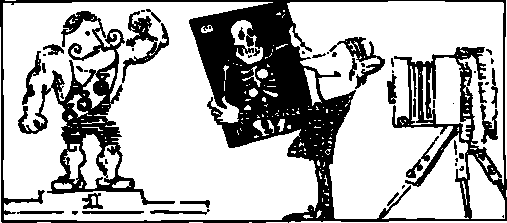
\includegraphics[width=\textwidth]{figures/fig-03-01.pdf}
%\caption{$X$-rays penetrate muscles and can show the skeleton.}
%\label{fig-3.1}
%\end{figure}

%
%%\newpage
%\begin{center}
%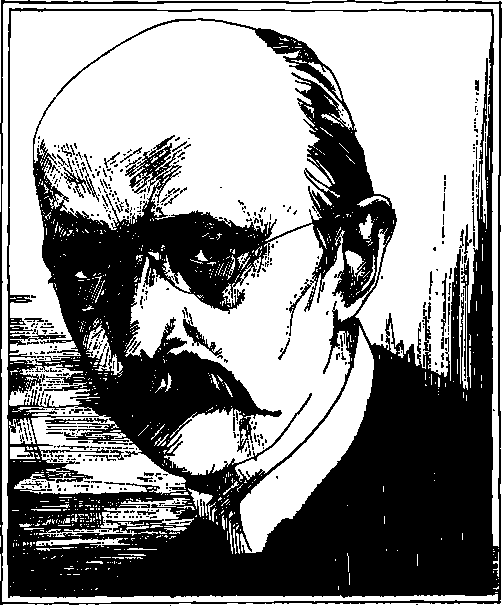
\includegraphics[width=\textwidth]{figures/planck.pdf}
%\end{center}
%{\small \textsf{\hlred{Albert Einstein [1879-1955]}} -- \textsf{\footnotesize the genius who created the theory of relativity and revolutionized all physical thinking. In 1905, Einstein published a treatise devoted to the special theory of relativity. In 1907, he obtained a formula relating energy and the mass of a body. In 1915, Einstein published his general theory of relativity. From this theory there followed new laws of gravita­tion and conclusions concerning the curvature of space.}}



